\documentclass[10pt,twocolumn,letter]{article}
\usepackage{styles/usenix-style}
\usepackage{styles/ka-style}
\usepackage{xspace,ifthen,graphicx,listings}
\usepackage{styles/ka-style}

\usepackage[utf8]{inputenc}
\usepackage[inline]{enumitem}
\usepackage{parskip} % disable indentation for new paragraphs, increased margin-bottom instead
\usepackage[english]{babel}
\usepackage{csquotes}
\usepackage[style=alphabetic]{biblatex}
\addbibresource{literature.bib}

\usepackage[
   pdfauthor={Christian Schwarz},
   pdftitle={Seminar Report - Light-Weight Contexts},
   pdfsubject={An OS Abstraction for Safety and Performance}, 
   pdfkeywords={}
]{hyperref}

\setlength{\marginparwidth}{2cm} % to make todonotes fit in twocolumn
\usepackage{todonotes}

\usepackage{blindtext}

\usepackage{listings}
\lstdefinestyle{lwcapi}{language=[ANSI]C,basicstyle=\ttfamily,basewidth=0.5em,fontadjust=true}
\lstset{style=lwcapi}

\begin{document}
\title{%
  % document class article doesn't support subtitles, let's hack them
  {\normalfont \normalsize Seminar Report on}\\%
  Light-weight Contexts\\%
  {\normalfont \normalsize An OS Abstraction for Safety and Performance}\\%
  {\normalfont \small %
    James Litton\textsuperscript{1,2}
    Anjo Vahldiek-Oberwagner\textsuperscript{2}
    Eslam Elnikety\textsuperscript{2}
    Deepak Garg\textsuperscript{2}
    Bobby Bhattacharjee\textsuperscript{1}
    Peter Druschel\textsuperscript{2}
  }\\
  {\normalfont \small
    \textsuperscript{1}University of Maryland, College Park 
    \textsuperscript{2}Max Planck Institute for Software Systems
  }%
}
\author{Report by Christian Schwarz}
\date{2019}

\maketitle

\begin{abstract}
  \blindtext
\end{abstract}

\section{Introduction}\label{intro}

Application Compartmentalization as in seminar presentation. Ignore Session Isolation \& Snapshots?

Line of throught:

Modern app architecture commonly emphasizes modularization \& information hiding (Parnas) to achieve testability, maintainability, exchangability, reusability.
The extreme of reusability are large libraries used by multiple independent applications.

However, chasm between development time and runtime:
PLs enforce encapsulation at compile time, but the resulting program runs in a single protection domain, i.e. a process, at runtime:
shared address space with shared heap, shared file descriptor table, shared system-level privilege (user id, group id, capabilities(SYS\_CAP\_), system call) between all modules of the program.
Consequently, an exploitable vulnerability in a single module not only compromises that module but the entire application.

The generic solution: decomponsition of the application into smaller units that execute in separate protection domains.
Generic questions / problems / tradeoffs:
\begin{itemize}
  \item threat model
  \item definition of what makes a protection domain
  \item how to integrate the decomposition into different protection domains into the PL / runtime?
  \item applicability to existing PLs \& code bases
  \item how to maintain application performance
\end{itemize}

\subsection{Structure of this Report}
\blindtext


\section{Design}\label{design}
We find it most helpful to develop the general idea of \textit{light-weight Contexts} (lwCs) by starting from the canonical abstraction of processes \& threads, as visualized in figure~\ref{design:fig:canonicalprocthreads}.
\begin{figure}
  \label{design:fig:canonicalprocthreads}
  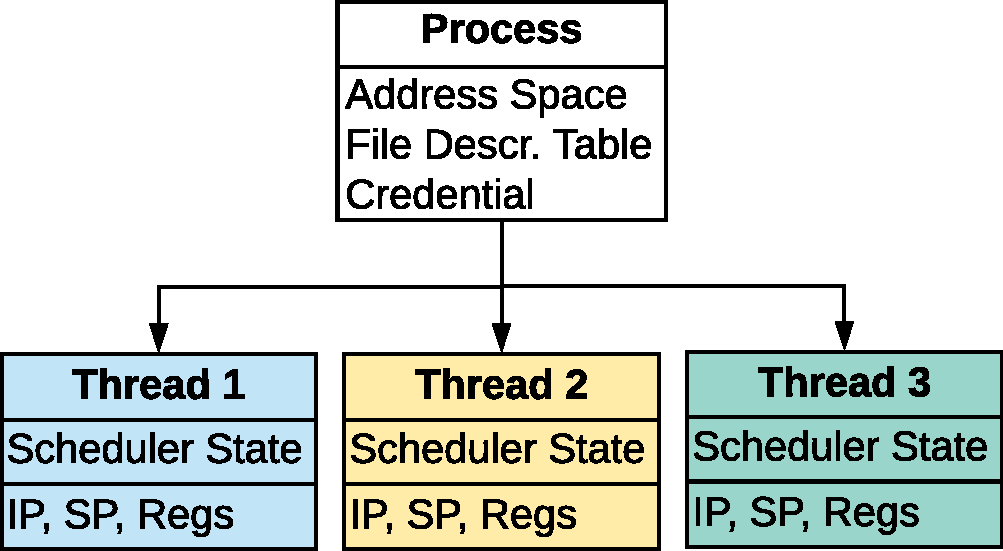
\includegraphics[width=\linewidth]{fig/canonical-proc-thread-relationship}
  \caption{
    Canonical state associated with processes and threads and the relationship between them.
    The process implicitly defines the execution environment for threads.
    Threads are scheduling entities that represent a single control flow bound to the process-defined environment.
  }
\end{figure}
Conventionally, processes define an execution environment which is shared by one or more threads.
The execution environment consists of an address space, a file descriptor table and a representation of the process's system-wide privileges (\textit{credential}).
A thread has \textbf{two closely related, but separate roles}:
\textbf{first}, it represents a \textbf{single unit of logical control flow} within the process-defined environment.
Control flow has associated state, e.g., instruction pointer, stack pointer, general purpose register contents, FPU state, etc.
That state resides in a CPU's registers while the thread is executing on a CPU, or in the thread control block (TCB) kernel data structure.
The \textbf{second} role of a thread is that of a \textbf{scheduling entity}:
The scheduler time-multiplexes threads onto CPU cores and implements the concept of blocking \& waiting between threads.
The scheduler state required for this task is stored in the thread control block (TCB).

The authors introduce light-weight contexts as a new OS abstraction and restructure the roles of canonical processes \& threads, as visualized in figure~\ref{design:fig:lwcprocthreadrelationship}:

\begin{figure}[h]
  \label{design:fig:lwcprocthreadrelationship}
  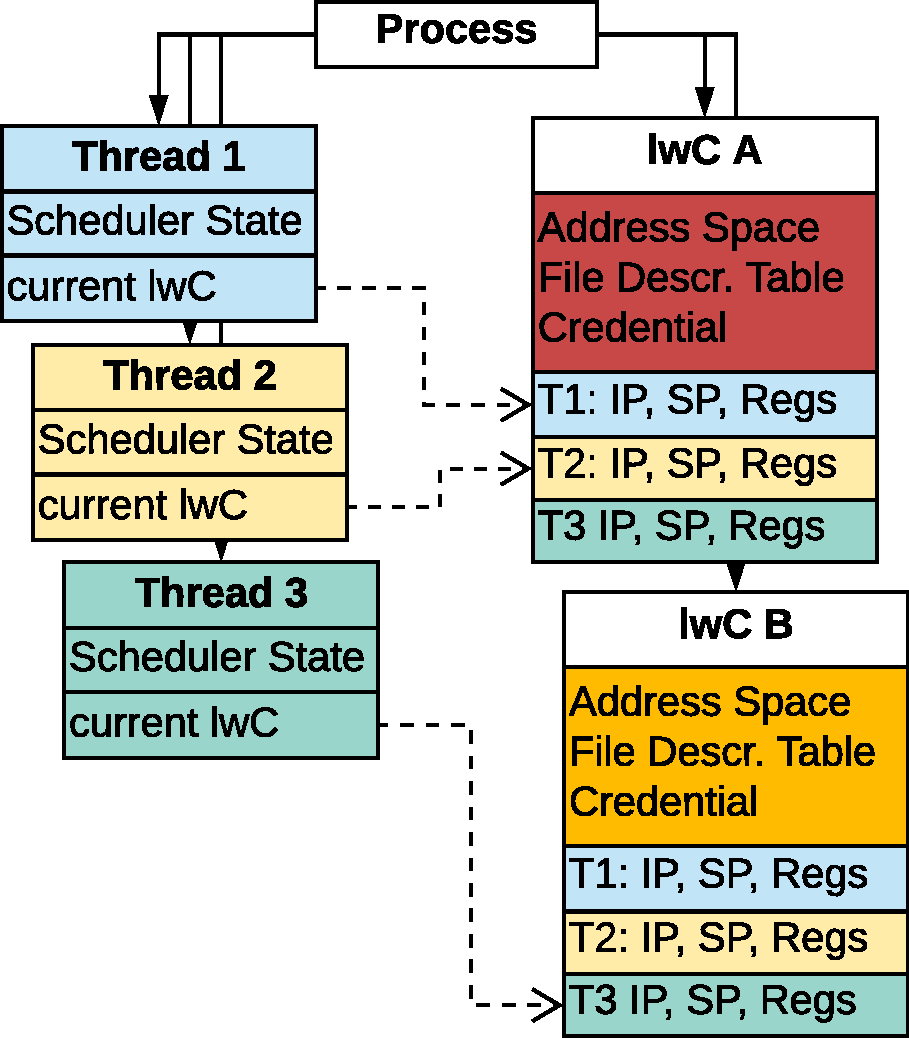
\includegraphics[width=\linewidth]{fig/lwc-proc-thread-relationship}
  \caption{
    State associated with lwCs, processes and threads and relationships between them.
    Processes act as containers for threads and lwCs.
    Threads are reduced to their role as scheduling entities.
    Each lwC represents an execution environment and holds control flow state for each thread.
  }
\end{figure}

\begin{itemize}
\item An lwC represents a single protection domain (address space, file descriptor table and system credential) and all logical control flows within that protection domain.
\item Threads always execute within one lwC at any given time and always execute the same logical control flow while within that lwC.
\item Multiple threads can execute simultaneously within an lwCs, sharing a protection domain but executing different logical flows.
\item lwCs are represented as file descriptors, and thus explicitly tangible from user space.
\item Threads can switch protection domains and logical control flow by switching between lwCs.
\end{itemize}

In the following subsections, we provide an outline of the system API for managing and using lwCs in an application.
Subsequently, we summarize the security guarantees provided by lwCs and provide usage examples for this new OS abstraction. 

\subsection{lwC Switching}\label{design:switching}
We start our survey of the lwC API surface with the most central functionality: switching between lwCs.
We accept the existence of multiple lwCs for now and come back to lwC creation in the next subsection.

Threads can switch between lwCs by invoking the \lstinline{lwcSwitch} system call:

\begin{lstlisting}[float=h]
  caller, carg := lwcSwitch(target, arg) 
\end{lstlisting}

The first argument \lstinline{target} specifies the file descriptor of the lwC into which the calling thread wants to switch.
When invoking the system call, the kernel
\begin{enumerate}[label=(\alph*)]
\item saves the current control flow state into the current thread's lwC,
\item atomically switches to the new protection domain by installing the target lwC address space, file descriptor table and credential for the current thread,
\item and restores the control flow state saved for the current in thread in the target lwC.
\end{enumerate}
Pseudo code for this procedure is provided in listing~\ref{design:fig:switchpseudocode}.

\begin{lstlisting}[mathescape,label=design:fig:switchpseudocode,caption=Pseudo code for lwcSwitch.,frame=trbl]
  syscall
  
  SP, IP, $\dots$ $\rightarrow$ curLWC->tcb[tid]
  
  curThd->vmspace = targetLWC->vmspace
  curThd->fdt = targetLWC->fdt
  curThd->cred = targetLWC->cred
  curLWC = targetLWC
  
  SP, IP, $\dots$ $\leftarrow$ targetLWC->tcb[tid]
  (arg kept in register)
  
  sysret  
\end{lstlisting}
  
It is crucial to understand that \textbf{execution after a switch always resumes at an lwC call site}, except for the very first switch into a newly created lwC (see section~\ref{design:createdestroy}).
Note that this behavior is analogous to a voluntary context switch, e.g., with \lstinline{pthread_yield}.
However, in contrast to the canonical model of processes \& threads, \textbf{\lstinline{lwcSwitch} does not switch to another scheduling entity}:
from the thread scheduler's perspective, it is still the same thread that is executing on the CPU.
In fact, \textbf{the thread scheduler is not affected at all by lwC switching}:
it still handles context switches post-interrupt, post-exception or when a thread blocks, by simply saving that thread's control flow state to the slot in the current lwC before switching to another thread (i.e.~scheduling entity).

The second argument to \lstinline{lwcSwitch} is an opaque value called \lstinline{arg} that is passed through to the code that starts executing in the target lwC after the switch is completed.
\lstinline{arg} is made available in the target lwC as the return value \lstinline{carg} (we remember that execution always resumes at an lwC call site).
The second return value \lstinline{caller} is the file descriptor of the lwC from where the switch was initiated.
Having this information available in the switch target enables subroutine-style usage of \lstinline{lwcSwitch} because it enables switching back to any number of callers that are unknown at compile time.

% do not mention coroutines here, will do that in the application

\subsection{lwC Creation \& Destruction}\label{design:createdestroy}
A process in an lwC system starts with a single thread that runs within a root lwC created by the OS.
This design enables backwards binary-compatiblity with the exception that the root lwC file descriptor is a well-known number analogous to those for stdio.

New lwCs can then be created by threads using the \lstinline{lwcCreate} system call:

\begin{lstlisting}[mathescape]
  rspecs :=
    [{Resource,[A, B), COPY|UNMAP|SHARE}, ...]
  new, caller, carg := lwcCreate(rspecs)
  /*              new      caller      carg
   *  creator   new lwC       0          0
   *  new lwC      0         like lwcSwitch
   */
\end{lstlisting}

By default, a new lwC is a snapshot of the calling thread's current lwC, as depicted in figure~\ref{design:fig:lwccreationsequencediagram}:
The kernel first creates copies of the resources \textit{address space, file descriptor table} and stores them in the new lwC.
It then temporarily preempts all threads that execute in the current lwC and stores their control flow state in the new lwC.
The execution state of other threads that can switch to the creating lwCs is simply copied to the new lwC.
Finally, the file descriptor referring to the new lwC is returned to user space in the return value \lstinline{new}.

\begin{figure}
  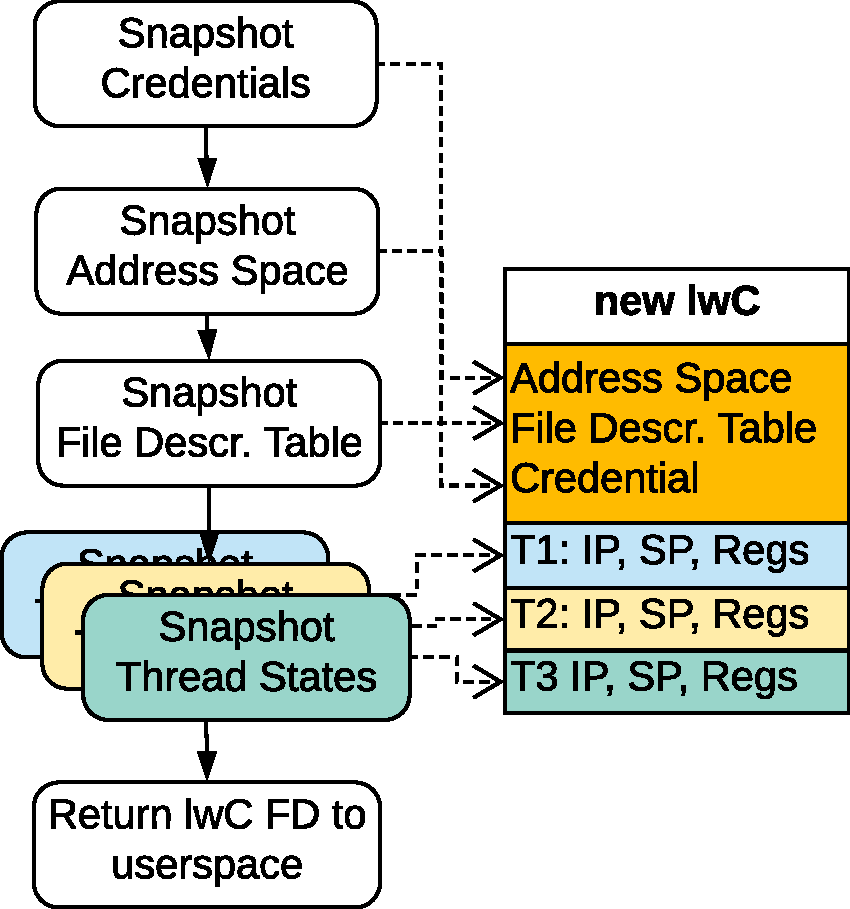
\includegraphics[width=\linewidth]{fig/lwc-creation-sequence-diagram}
  \caption{
    Steps involved in lwC creation.
    By default, a new lwC is a copy (snapshot) of the current lwC's resources.
    All threads that exist at the time of lwC creation can enter the new lwC.
  }
\label{design:fig:lwccreationsequencediagram}
\end{figure}

Note that in contrast to the original paper, we avoid the term \textit{fork} when describing the lwC creation procedure:
forking has the same resource snapshotting semantics as \textit{lwcCreate}, but also implies the creation of a new process and scheduling entity.
In contrast, \textit{lwcCreate} only creates a copy of the protection domain and a handle for existing threads to switch to it.

However, there is still overlap with fork semantics and the problems associated with this artifact of early UNIX history: % TODO ref microsoft paper
\textbf{what happens when we first switch into a newly created lwC?}
After all, we preempt and snapshot all threads' control flow states on lwC creation, and the \lstinline{lwcSwitch} implementation restores that state on first switch, expecting that it was an \lstinline{lwcSwitch} call site.
The \lstinline{lwcCreate}ing thread will appear return "a second time" from that syscall.
The \lstinline{lwcSwitch} return values can thus be made available in \lstinline{lwcCreate}'s \lstinline{caller} and \lstinline{carg} variables.
Other threads could be at random points in the logical control flow they were executing, resulting in undefined behavior after the switch.\todo{obvious?}
Multithreaded forking is a well-known problem, \todo{citations} and the authors recommend applications to use barrier-synchronization with the creator.\todo{cite}
However, it is unclear to us how the \lstinline{caller} and \lstinline{carg} return values are accessible without inline-assembly or language support for non-creator threads.\todo{check}

\subsubsection{lwC Resource Specifiers}\label{design:rspecs}

% TODO What about SysV IPC, other shared namespaces? => systrap mechanism?
The only argument to \lstinline{lwcCreate} is \lstinline{rspecs}  

\subsubsection{Static Resource Sharing}

\subsection{Dynamic Resource Sharing with lwC Overlays}\label{design:overlays}

\subsection{Syscall Interposition}\label{design:syscallinterpos}

\subsection{Threat Model \& Security Guarantees}\label{design:threat}

\subsection{Usage Examples}\label{design:usage}

\subsection{Limitations}

\section{Implementation \& Evaluation}\label{eval}

\subsection{Critique}\label{eval:crit}

\section{Related Work}\label{rel}

\begin{itemize}
  \item Application Compartmentalization
  \begin{itemize}
    \item Principle of least Privilege
    
    \item Language-Technology-Based
    \begin{itemize}
      \item NaCL \& WASM
      \item BPF \& eBPF
      \item Software Fault Isolation
      \item Memory-safe Runtime (Java, CLR?) %working title, need proper PL word for it
    \end{itemize}
    
    \item OS-Based
      \begin{itemize}
        \item Capability Systems
        \begin{itemize}
          \item Fiasco-OC / seL4
          \item FreeBSD Capsicum
        \end{itemize}
        \item Process-Based Privsep
        \begin{itemize}
          \item Provos, OpenSSH
        \end{itemize}
        \item Hybrids (isolation at some level)
        \begin{itemize}
          \item wedge
          \item shreds (uses ARM memory domains)
          \item \textbf{light weight contexts}
        \end{itemize}
      \end{itemize}

    \item Hardware-Based
    \begin{itemize}
      \item CHERI
    \end{itemize}
  \end{itemize}
  
  \item Process Snapshotting \& Rollback
  \item Session Isolation in CGI applications?
\end{itemize}

\section{Conclusion}\label{conclusion}

% Cite all the literature, not just the one we referenced in the text.
\nocite{*}
\clearpage
\printbibliography

\end{document}
